\chapter{Validation}
\label{sec:validation}
To verify that the prototype conforms to the design in chapter \ref{sec:design}, the prototype has been tested with automatic unit tests and manual system tests.
As described in the implementation chapter the unit tests are part of the continuous integration toolchain and are automatically run when a new merge request is created.
The system tests are of a more manual nature and have been conducted according to the test specifications defined in this chapter.

\section{Unit tests}
To implement the unit tests, Go's default testing framework has been used.
This framework has been setup as part of the continuous integration checks so that a failing test is not missed when a merge request is made.
At the time of writing this section, most of the code concerning the templates and parameters is covered by unit tests and all of these pass.
However the percentage of code covered by unit tests is still below the required 90\%.
This means that there still might be some edge cases that have not been handled but the correct operation is also verified by the system tests in the next section.
The expectation is that this percentage will improve between the completion of this thesis and the presentation.
The final results of the unit tests will be presented at this time.

It was difficult to get good code coverage for the components of the prototype that interacted with the camera's over HTTP because the utilized testing framework did not provide an ability to mock HTTP responses.
In the last weeks of the project a possible method of testing this code was found that implemented a HTTP server that pretended to be a camera.
However with the time that remained it was decided not to implement a separate HTTP server as this code could also be tested satisfactorily by the system tests.
This method of testing might still be of interest in the future and has been included as a recommendation in chapter \ref{sec:recommendations}.

\section{System test}
To test the parts of the application that could not be covered by unit tests manual system tests have been performed.
The test specifications will list what requirements they test, what the test procedure is and what results indicate a passed test.
These tests are used to determine if all requirements have been satisfied and to verify behavior of components that could not be unit tested.
These system tests have been done in the last week of the project to most closely resemble the state of the application.

System tests have been defined with the following information: a short name indicating the purpose of the test, a test description, a list of requirements being tested, and the results of the test.

\begin{marginfigure}
	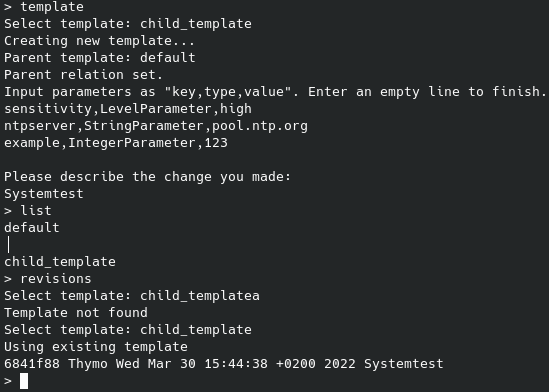
\includegraphics{manage_template}
	\caption{System test 1 result}
	\label{test:2}
\end{marginfigure}

\begin{test}[label={test_camera}]{Managing a template}
	The application should be able to add new templates and configure parameters.
\tcbline
	\begin{description}
		\item[Requirements:] B1, B4, U3, U5, U6, U7, NF8
		\item[Test passes when:] \hfill
			\begin{itemize}
				\item Template can be created.
				\item Parameters can be added to a template.
				\item Template can have a parent associated with it.
				\item Changes are saved inside a revision.
			\end{itemize}
		\item[Result:] Passed (Figure \ref{test:2})
	\end{description}
\end{test}

\begin{marginfigure}
	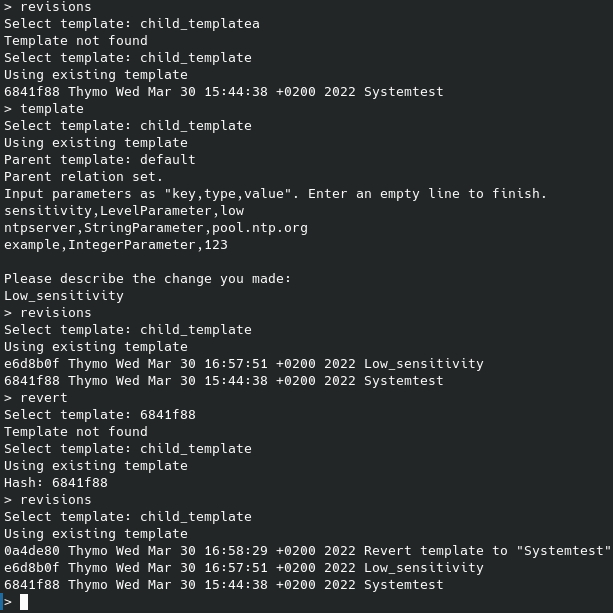
\includegraphics{revert}
	\caption{System test 2 result}
	\label{test:3}
\end{marginfigure}

\begin{test}[label={test_camera}]{Reverting a template}
It should be able to revert a template to a previous revision.\\
\tcbline
	\begin{description}
		\item[Requirements:] B2, B3, U2
		\item[Test passes when:] \hfill
			\begin{itemize}
				\item Revisions and audit information of a template can be displayed.
				\item A new revision can be made by editing a template.
				\item A template can be reverted to an earlier revision.
			\end{itemize}
		\item[Result:] Passed (Figure \ref{test:3})
	\end{description}
\end{test}

\begin{marginfigure}
	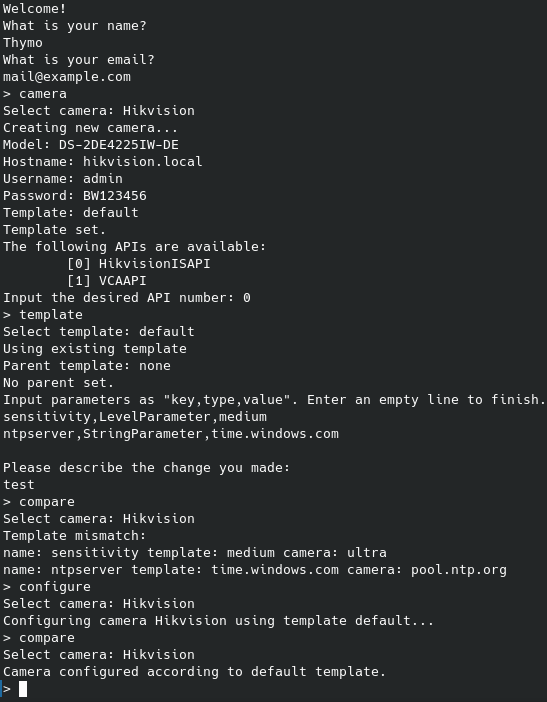
\includegraphics{hikvision_configure}
	\caption{System test 3 result}
	\label{test:4}
\end{marginfigure}

\begin{test}[label={test_hikvision}]{Hikvision support}
It should be possible to read and write the NTP and motion detection sensitivity parameters from the Hikvision camera.
Using this information the compare command should show any mismatches with the template and allow for these to be corrected using the configure command.
\tcbline
	\begin{description}
		\item[Requirements:] B1, B4, B5, U3, U7, U8, U9, NF1, NF8
		\item[Test passes when:] \hfill
			\begin{itemize}
				\item Two parameters supported by the camera can be set in a template.
				\item A mismatch is displayed when the camera value differs from the template.
				\item The parameters from the template can be transferred using the configure command.
				\item Proper updating of the parameters is confirmed by a second compare command.
			\end{itemize}
		\item[Result:] Passed (Figure \ref{test:4})
	\end{description}
\end{test}

\begin{marginfigure}
	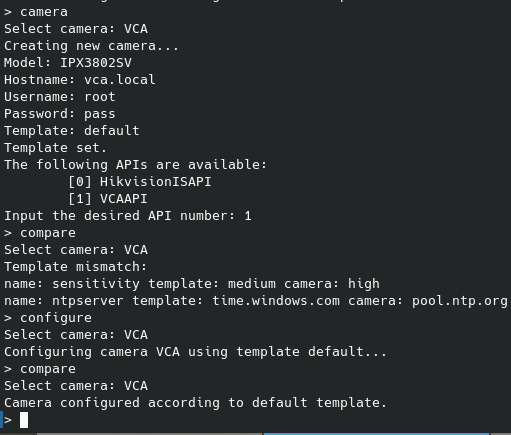
\includegraphics{vca_configure}
	\caption{System test 4 result}
	\label{test:5}
\end{marginfigure}

\begin{test}[label={test_vca}]{VCA support}
It should be possible to read and write the NTP and motion detection sensitivity parameters from the Hikvision camera.
Using this information the compare command should show any mismatches with the template and allow for these to be corrected using the configure command.
\tcbline
	\begin{description}
		\item[Requirements:] B1, B4, B5, U3, U7, U8, U9, NF1, NF8
		\item[Test passes when:] \hfill
			\begin{itemize}
				\item Two parameters supported by the camera can be set in a template.
				\item A mismatch is displayed when the camera value differs from the template.
				\item The parameters from the template can be transferred using the configure command.
				\item Proper updating of the parameters is confirmed by a second compare command.
			\end{itemize}
		\item[Result:] Passed (Figure \ref{test:5})
	\end{description}
\end{test}

\begin{marginfigure}
	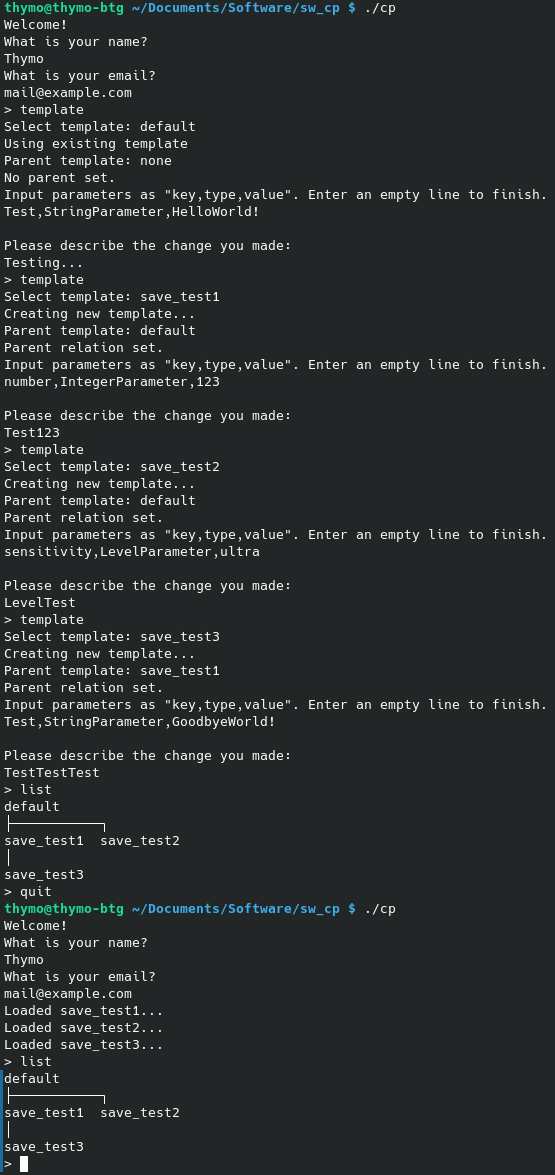
\includegraphics{test_reload}
	\caption{System test 5 results}
	\label{test:6}
\end{marginfigure}

\begin{test}[label={test_camera}]{Saving and loading}
The application should be able to reload the templates that were previously saved when the application is started.
\tcbline
	\begin{description}
		\item[Requirements:] NF6, NF8
		\item[Test passes when:] \hfill
			\begin{itemize}
				\item Multiple templates containing a parameter are created.
				\item Template hierarchy can be shown before and after restarting the program.
				\item Templates are automatically reloaded.
				\item Hierarchy is preserved across restarts.
			\end{itemize}
		\item[Result:] Passed (Figure \ref{test:6})
	\end{description}
\end{test}


\section{Demonstration}
To demonstrate the operation of the application a demonstration of the possible commands will be shown.

\subsection{author}
When the application is started or on the invocation of the `author` command the user is asked to enter their name and email address as seen in figure \ref{demo_author}.
This information is used when a new template revision is made so that this information is available for auditing purposes when listing a template's revisions.
\begin{marginfigure}
	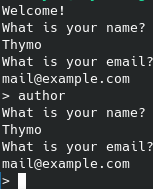
\includegraphics[scale=0.5]{author}
	\caption{Entering author information}
	\label{demo_author}
\end{marginfigure}

\subsection{camera}
The camera command can be invoked by the user to create a new camera or to edit an existing camera.
Upon entering the desired camera name the application will try to find a camera with this name to edit or create a new camera if one can not be found.
Once this is done the user is asked a couple of questions so the application knows how to interact with the camera and what template it should use.
In addition, the list\_cameras command can be used to show a list of cameras registered with the application.
An example is show in figure \ref{demo:camera}.
\begin{marginfigure}
	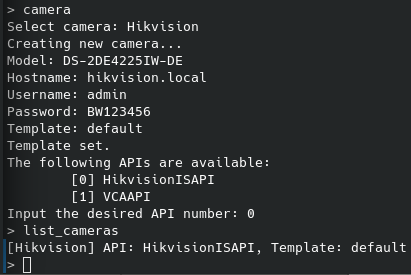
\includegraphics{camera}
	\caption{Creating a new camera}
	\label{demo:camera}
\end{marginfigure}

\subsection{template}
The template command is used to create or edit a template as seen in figure \ref{template}.
Same as the camera command the template command will try to find an already existing template and if none can be found one will be created.
After that the application will ask what the parent of this template should be.
If a template can not be found the question is repeated until an existing template is found.
An exception is made when editing the default template.
Since this template is the root node of the tree it has no parents and the only accepted value is 'none'.
A value of 'none' is not accepted for other templates,

\begin{marginfigure}
	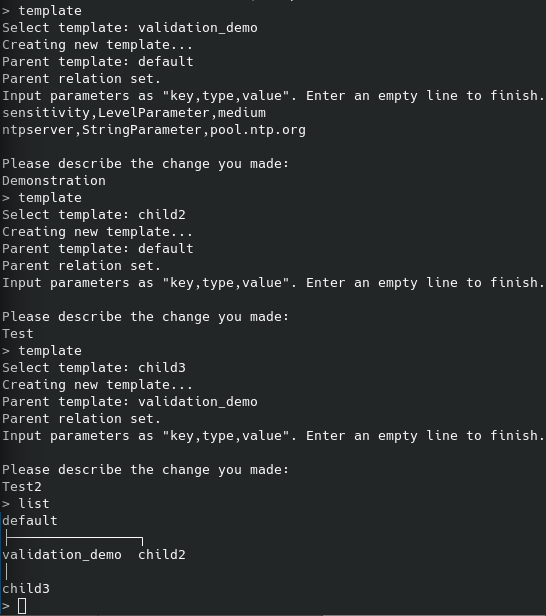
\includegraphics{template}
	\caption{Creating templates and showing the tree}
	\label{template}
\end{marginfigure}

\subsection{revisions \& revert}
Templates can also be reverted to an earlier revision and a log of when and why they were changed by someone can also be displayed.
For this the `revisions` and `revert` commands have been provided (Figure \ref{revisions}).
The revisions command will display a list of all revisions of a particular template.
This list contains a 7 character commit hash, the name of the author, a timestamp and a message about the change.
In order to revert a template to an earlier revision, the `revert` command can be used.
When the user supplies the name of the template and the commit hash of an earlier revision, that template will be reset to the state at that point in time.
A new revision is created from this showing to what point the template was reverted without permanently destroying the revisions.
This way the user can still decide to undo the reversion if they supply the hash of a newer revision.

\begin{marginfigure}
	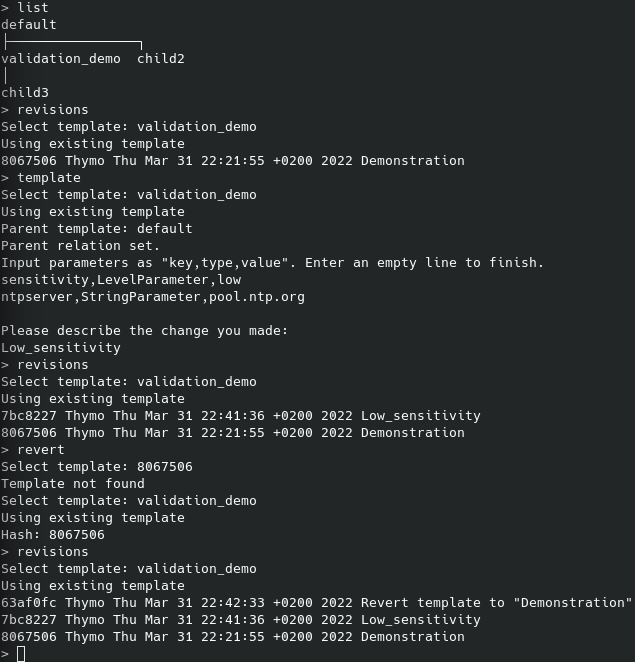
\includegraphics{revisions}
	\caption{Editing a template and reverting it to a previous revision}
	\label{revisions}
\end{marginfigure}

\subsection{compare}
To compare the current state of a camera to the parameters it should have according to the assigned template the `compare` command can be used.
As seen in figures \ref{test:4} and \ref{test:5} this will query the requested camera and compare the parameters from the template to the ones from the camera.
When there are no mismatches no parameters will be listed, only mismatches will be shown to the user.

\subsection{configure}
The settings of a camera can be updated by using the `configure` command.
This command will translate the parameters from the template to camera specific values and will send them to the camera as seen in figures \ref{test:4} and \ref{test:5}.

\subsection{list \& list\_cameras}
The `list` and `list\_cameras` command will show an overview of all templates and cameras respectively.
When the user requests a list of the templates their names will be shown with lines in between them to show the hierarchy of the complete tree.
The `list\_cameras` command shows the name of the camera, the API it uses and what template it is using.
